
\definecolor{green}{RGB}{0,128,0}
  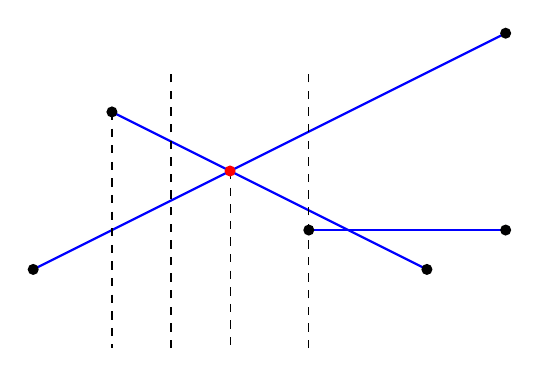
\begin{tikzpicture}
    % Define the points
    \coordinate (A) at (1, 1); 
    \coordinate (B) at (7,4 );
    \coordinate (C) at (2, 3); 
    \coordinate (D) at (6,1 );
    \coordinate (E) at (4.5, 1.5); 
    \coordinate (F) at (7, 1.5);

    \coordinate(C1) at (2, 0);
    \coordinate(I) at (3.5, 2.25);
    \coordinate(I1) at (3.5, 0);
    \coordinate(E1) at (4.5, 0);
    \coordinate(E2) at (4.5, 3.5); 

    \coordinate(R1) at (2.75, 0);
    \coordinate(R2) at (2.75, 3.5); 
    
    \draw[thick, blue] (A) -- (B);
    \draw[thick, blue] (C) -- (D);
    \draw[thick, blue] (E) -- (F);
    % Draw the points
    \foreach \point in {A,B,C,D,E,F}
      \fill (\point) circle (2pt);

    % \foreach \point in {A,B,C,D,E,F, I}
    %   \node[above right] at (\point) {\point};

    \onslide<2>{
        \draw[dashed, black] (C) -- (C1);
        \draw[dashed, black] (E1) -- (E2);
    }
        
    \onslide<2-3>\draw[dashed, black] (I) -- (I1);

    \onslide<3-> \fill[red] (I) circle (2pt);
    \onslide<4> {
        \draw[dashed, black] (R1) -- (R2);
    }


    % \node[above right] at (B) {B};
    % \node[above right] at (C) {C};
    % \node[above right] at (D) {D};
    % \node[above right] at (E) {E};
    % \node[above right] at (F) {F};
    % \node[above right] at (G) {G};
    % \node[above right] at (H) {H};

    
    % Draw the convex hull
    
    

  \end{tikzpicture}
